% DOCUMENT
\documentclass[oneside,14pt,a4paper]{extreport}

% LANGUAGE
\usepackage[T2A]{fontenc}
\usepackage[utf8]{inputenc}
\usepackage[english, ukrainian]{babel}

% \usepackage{minted}
\usepackage{pgfplots}

% VARIABLES
\newcommand \labno    {3}
\newcommand \course   {Організація наукових досліджень}
\newcommand \group    {11}
\newcommand \lecturer {Ізонін І. В.}
\newcommand \theme    {Пошук наукової літератури за допомогою спеціалізованих пошукових систем та бібліографічних баз}
\newcommand \purpose  {Навчитися здійснювати пошук наукової літератури за допомогою спеціалізованих пошукових систем та бібліографічних баз (Scopus, Google Академія) згідно тематики дипломної роботи.}

% PACKAGES
\usepackage{amssymb}
\usepackage{amsmath}
\usepackage{multirow}
\usepackage{url}
\usepackage[unicode=true]{hyperref}
\usepackage{hanging}

% GEOMETRY
\usepackage{geometry}
\geometry{left   = 2.5cm}
\geometry{right  = 1cm}
\geometry{top    = 2cm}
\geometry{bottom = 2cm}
\renewcommand {\baselinestretch} {1.5}
\setlength\parindent{1cm}

% IMAGES
\usepackage{graphicx}
\usepackage{indentfirst}
\graphicspath{ {./imgs/} }
\usepackage{float}

% FOOTER
\usepackage{fancyhdr}
\fancyhf{}
\renewcommand{\headrulewidth}{0pt}
\cfoot{\hfill \thepage}
\pagestyle{fancy}

% CHAPTERS

\newcommand\Section[1]{
 \refstepcounter{section}
 \section*{
  \arabic{section}. #1}
}

\newcommand\Subsection[1]{
 \refstepcounter{subsection}
 \section*{
  \arabic{section}.\arabic{subsection}. #1}
}

\sloppy
\begin{document}
\begin{titlepage}

\centering
 \textbf{
  МІНІСТЕРСТВО ОСВІТИ І НАУКИ УКРАЇНИ \
  НАЦІОНАЛЬНИЙ УНІВЕРСИТЕТ \flqq{}ЛЬВІВСЬКА ПОЛІТЕХНІКА\frqq{} \
  ІНСТИТУТ КОМП’ЮТЕРНИХ НАУК ТА ІНФОРМАЦІЙНИХ ТЕХНОЛОГІЙ
 }

\vspace{0.5cm}
 \textbf{
  Кафедра систем штучного інтелекту
}

\vspace*{\fill}

  {
    \centering
    
\includegraphics[width=7cm]{imgs/logo.eps}
  }

\vspace{1cm}

  {\textbf{ЗВІТ} \par{}
  {про виконання практичної роботи №\labno}
   \par}
  {з курсу \flqq{}\course\frqq{} \par}

\vspace{1cm} \theme

\raggedleft\vfill

 {\textbf{Виконав:} \par}
 {ст. гр. КНСШ-\group \par}
 {Тимошенко Павло Олександрович \par}

% \vspace{1cm}

 {\textbf{Перевірив:} \par}
 {доцент каф. СШІ, к.т.н.,}
 {\lecturer \par}

\vspace{1cm}

\centering {Львів -- \the\year \par}

\end{titlepage}

\Section{Постановка завдання}

Далі описано пункти, які потрібно виконати у межах цієї практичної роботи.

\begin{enumerate}
    \item Написати тему та мету дипломної роботи, при можливості об'єкт та предмет дослідження. Визначити та оформити у таблицю 3-6 ключових слів, які найбіль повно можуть описати тематику.
    \item Знайти не менше трьох найбільш цитованих статей за темою роботи у бібліометричній базі даних Google Scholar (українською мовою). Включити у пошук лише статті, які опубліковано у 2020 році. Виключити із пошуку патенти та посилання. Додати знайдені роботи у Zotero.
    \item На основі обраних ключових слів сформувати пошуковий запит в наукометричній базі Scopus. Отриманий набір робіт зменшити із використанням наступних критеріїв:
    \begin{itemize}
        \item публікації лише з відкритим доступом;
        \item тип документу -- лише статті (а не тези конференції);
        \item документи лише англійською;
        \item публікації за останні три роки.
    \end{itemize}
    \item Здійснити опис проведеної роботи.
\end{enumerate}

\Section{Хід роботи}

В цьому розділі описано процес виконання практичної роботи та пророблені кроки. 

Тема дослідження: Використання та оптимізація алгоритму Вітербі при визначення частин мови в тексті українскою.

Мета дослідження:

\begin{itemize}
    \item розкрити застосовність алгоритму Вітербі до текстів українською;
    \item з'ясувати, чи цей алгоритм буде так само надійним, як і в аналізі тексту англійською, де його використали вперше;
    \item розробити надійний та швидкий спосіб використання алгоритму на тих словах, на яких не проводилось навчання;
    \item виявити надоліки алгоритму та продемонструвати можливі способи оптимізації.
\end{itemize}

Звідси можна сформувати такі ключові слова: \textit{алгоритм Вітербі} (англ. \textit{Viterbi algorithm}), \textit{NLP}, \textit{розмітка частин мови} (англ. \textit{POS tagging}), \textit{українська мова} (англ. \textit{Ukrainian language}).

\Subsection{Пошук в Google Scholar}

Сформовані запити пошуку в Google Scholar показано на Рис.~\ref{pic:scholar1} та Рис.~\ref{pic:scholar2}.

\begin{figure}[t]
    \centering
    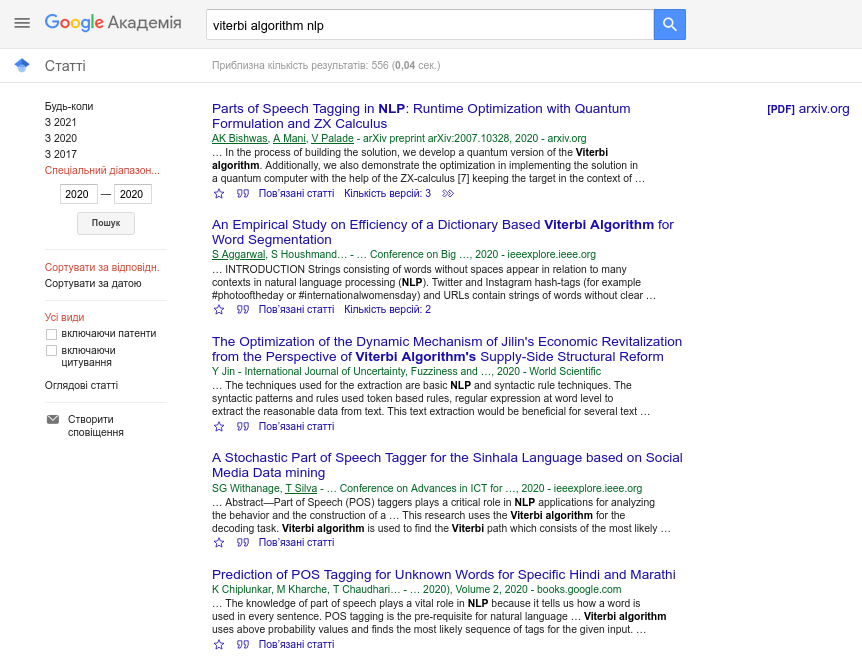
\includegraphics[width=\textwidth]{imgs/3_scholar_search_1.png}
    \caption{Пошуковий запит у Google Scholar з текстом \flqq{}pos tagging ukrainian\frqq{}}
    \label{pic:scholar1}
\end{figure}

\begin{figure}[t]
    \centering
    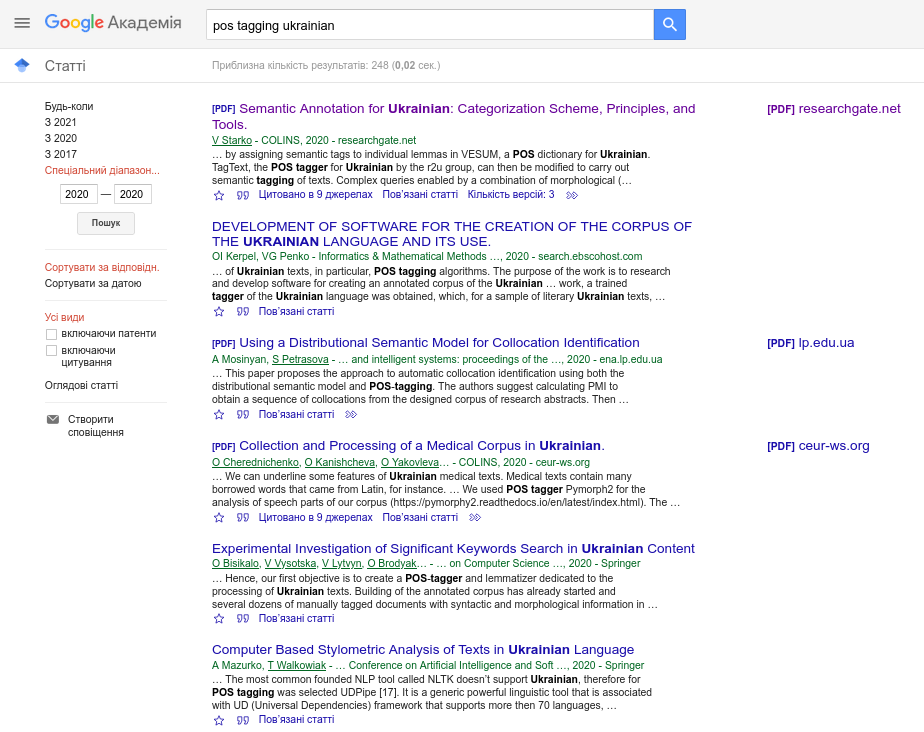
\includegraphics[width=\textwidth]{imgs/3_scholar_search_2.png}
    \caption{Пошуковий запит у Google Scholar з текстом \flqq{}viterbi algorithm nlp\frqq{}}
    \label{pic:scholar2}
\end{figure}

Посилання на знайдені статті подано далі:

\begin{enumerate}
    \item \url{https://www.researchgate.net/profile/Vasyl-Starko/publication/344841042_Semantic_Annotation_for_Ukrainian_Categorization_Scheme_Principles_and_Tools/links/5f92d758458515b7cf96d83c/Semantic-Annotation-for-Ukrainian-Categorization-Scheme-Principles-and-Tools.pdf} (цитовано в 9 джерелах);
    \item \url{http://ceur-ws.org/Vol-2604/paper21.pdf} (цитовано в 9 джерелах);
    \item \url{https://www.emerald.com/insight/content/doi/10.1016/j.aci.2018.12.003/full/html?utm_source=rss&utm_medium=feed&utm_campaign=rss_journalLatest} (цитовано в 8 джерелах).
\end{enumerate}

\Subsection{Пошук в Scopus}

Для пошуку в Scopus я сформував такий запит: \texttt{TITLE-ABS-KEY ( ( "pos"  OR  nlp )  AND  "viterbi algorithm" )  AND  PUBYEAR  >  2019  AND  ( LIMIT-TO ( DOCTYPE ,  "ar" ) )  AND  ( LIMIT-TO ( LANGUAGE ,  "English" ) )  AND  (  LIMIT-TO ( OA ,  "all" ) )}.

Обрані статті є 4, 5 та 6-ою позицією в бібліографії наступного розділу.

\Subsection{Сформована бібліографія}

Обрані статті я додав у Zotero. На Рис.~\ref{pic:zotero} показано вигляд вікна зі статтями. На Рис.~\ref{pic:ieee} подана сформована у стилі IEEE бібліографія.

\begin{figure}[H]
    \centering
    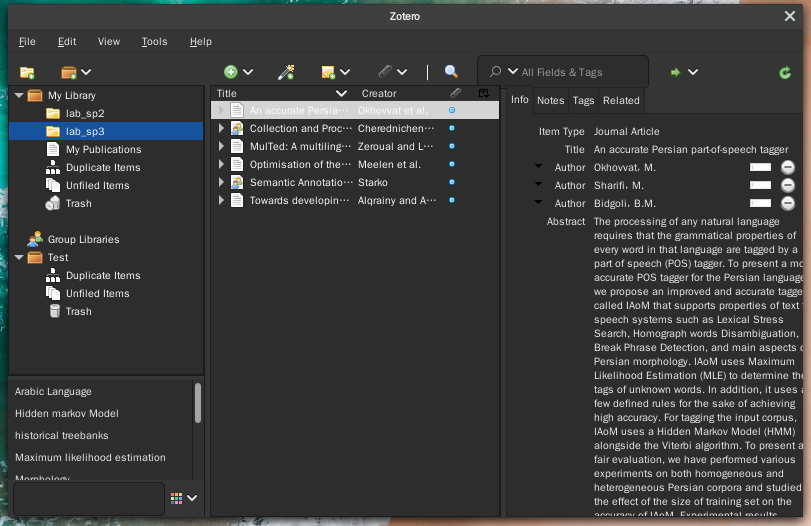
\includegraphics[width=\textwidth]{imgs/3_zotero.png}
    \caption{Вікно Zotero з доданими статтями.}
    \label{pic:zotero}
\end{figure}

\begin{figure}[H]
    \centering
    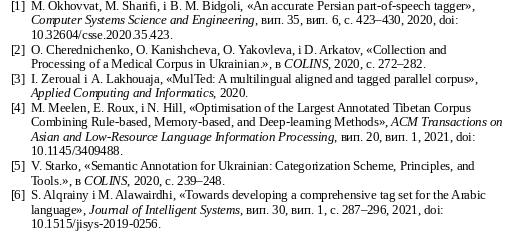
\includegraphics[width=\textwidth]{imgs/3_ieee.png}
    \caption{Сформована бібліграфія.}
    \label{pic:ieee}
\end{figure}

\Section{Результати та висновки}

У цій практичній роботі я сформував список ключових слів на основі поданої теми та мети дослідження. За ключовими словами я знайшов 6 статей у каталогах Google Scholar та Scopus, використовуючи не тільки текстуальний пошук, але й змінюючи категорії. Окрім того я навчися будувати пошуковий запит у системі Scopus.

Отримані вміння є важливими при написанні наукової роботі, оскільки дозволяють знайти інші праці на схожу тематику та посилатись на них. Це допоможе мені у написанні дипломної роботи.

\Section{Список використаної літератури}

\begin{enumerate}
\item Пошукова та наукометрична система Гугл Академія (Google Scholar)  [Електронний ресурс] – Режим доступу: 
\url{http://dnsgb.com.ua/files/%D0%A1%D0%98%D0%A1%D0%A2%D0%95%D0%9C%D0%90%20GOOGLE%20%D0%90%D0%9A%D0%90%D0%94%D0%95%D0%9C%D0%86%D0%AF.pdf} (відвідано 08.11.2020)
\item Веб-адреса бази даних Google Scholar. [Електронний ресурс] – Режим доступу: \url{https://scholar.google.com/} (відвідано 08.11.2020) 
\item Scopus – докладна інструкція для вченого [Електронний ресурс] – Режим доступу: \url{https://ua.publ.science/uk/blog/scopus---podrobnaya-instruktsiya-dlya-uchenogo} (відвідано 08.11.2020)
\end{enumerate}

\end{document}
